% !TeX spellcheck = en_US
\chapter{QUADRO TEÓRICO}

\par Neste capítulo serão discutidas as técnicas, metodologias e tecnologias que serão utilizadas no desenvolvimento deste trabalho.

\subsection{Iconix}

\par O Iconix foi escolhido como a metodologia de desenvolvimento de \textit{software}, desempenhando um papel fundamental na organização. Sua abordagem proveu uma sequência de procedimentos, levando à construção de uma aplicação estável. Como relatado no quadro teórico, foram seguidas as quatro fases definidas pelo Iconix,

\par Na primeira fase, definida como análise de requisitos, foi realizado o levantamento das informações pertinentes ao desenvolvimento. Este levantamento foi realizado por meio da observação do comportamento das pessoas ao buscar por mão de obra temporária. A partir daí, foram levantadas as principais características, indispensáveis para a construção do \textit{software} e desenvolvido o modelo de domínio inicial, como demonstra a Figura~\ref{fig:modelo_dominio_inicial}.

\newpage
\begin{figure}[h!]
	\centerline{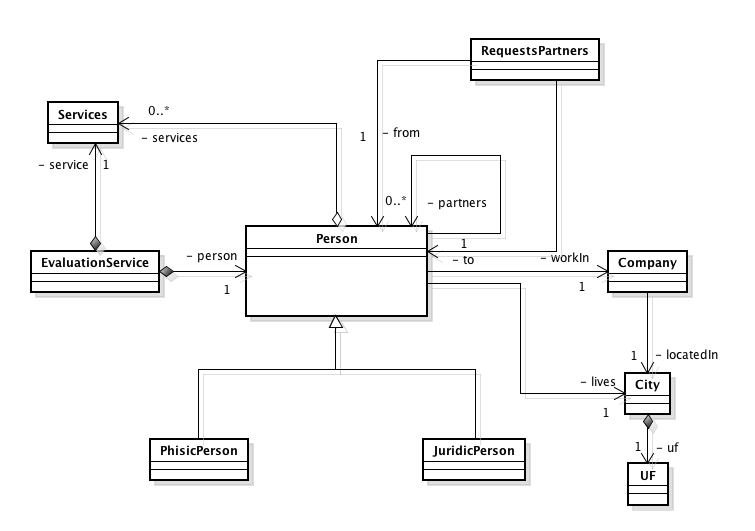
\includegraphics[scale=0.45]{./imagens/modelo-dominio-inicial.png}}
	\caption[Modelo de domínio inicial]
	{Modelo de domínio inicial. \textbf{Fonte:} Elaborado pelos autores.}
	\label{fig:modelo_dominio_inicial}
\end{figure}

\par Nesta fase, também foram definidas todas as ações cujo usuário poderia realizar no sistema, por meio dos casos de uso, conforme a Figura~\ref{fig:caso_uso_unificado}.

\newpage
\begin{figure}[h!]
	\centerline{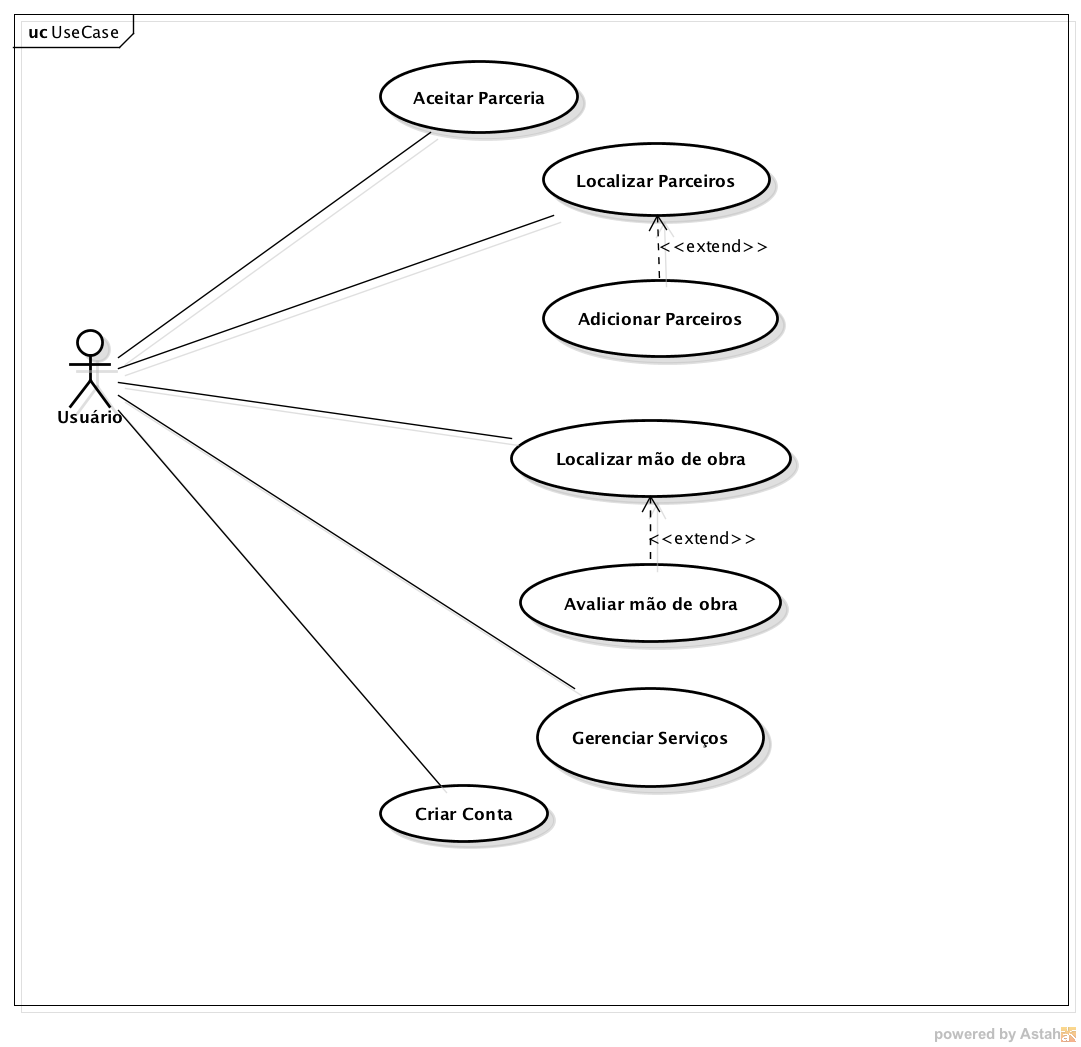
\includegraphics[scale=0.5]{./imagens/caso-de-uso-unificado.png}}
	\caption[Diagrama de caso de uso]
	{Diagrama de caso de uso. \textbf{Fonte:} Elaborado pelos autores.}
	\label{fig:caso_uso_unificado}
\end{figure}

% Removido após a pré-banca, pois, agora só haverá apenas um tipo de usuário (Ambos) e não mais provedor de serviço e contratante
%\newpage
%\begin{figure}[h!]
%	\centerline{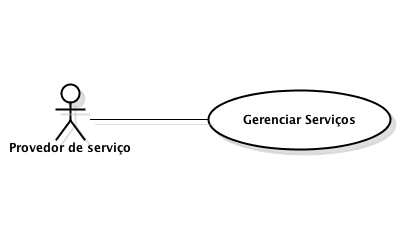
\includegraphics[scale=0.6]{./imagens/caso-de-uso-provedores-servico.png}}
%	\caption[Diagrama de caso de uso para provedores de serviços]
%	{Diagrama de caso de uso para provedores de serviços. \textbf{Fonte:} Elaborado pelos autores.}
%	\label{fig:caso_uso_provedor_servico_inicial}
%\end{figure}

%\begin{figure}[h!]
%	\centerline{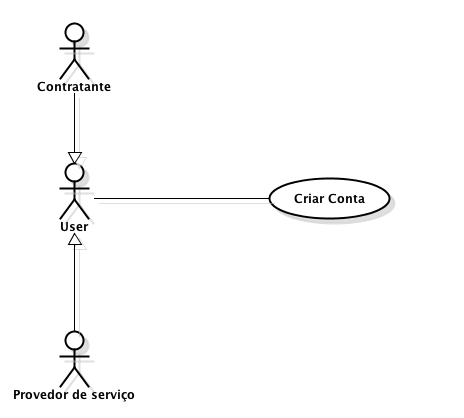
\includegraphics[scale=0.6]{./imagens/caso-de-uso-usuario.png}}
%	\caption[Diagrama de caso de uso para contratantes e provedores de serviços]
%	{Diagrama de caso de uso para contratantes e provedores de serviços. \textbf{Fonte:} Elaborado pelos autores.}
%	\label{fig:caso_uso_usuario_inicial}
%\end{figure}

\par Após definir os casos de uso, foram escritos os fluxos de eventos, para cada caso de uso. A seguir será apresentado o fluxo de eventos relacionado ao caso de uso ''Localizar parceiros'' por meio do Quadro~\ref{quad:fluxo_evento_localizar_parceiro}. Os demais fluxos de eventos são apresentados no Apêndice I em conjunto com os outros digramas deste trabalho.

% Conferir com o Márcio se os quadros serão removidos daqui e colocados nos apêndices depois só colar esta parte onde for inserida
%\newpage
%\begin{quadro}[h!]
%	\begin{fluxoDeEventos}
  \addTitle{Localizar Mão de obra}
  \addrow{Ator principal}{Contratante ou Ambos}
  \addrow{Ator secundário}{-}
  \addrow{Pré-condições}{O ator estar autenticado no sistema}
  \addrow{Pós-condições}{Provedores de serviço e suas respectivas mão de obras apresentadas ao ator.}
  
  \startBasicFlow{Ator} {Sistema}
  \addItemByColumnOne{O ator acessa a página para buscar o serviço por meio do menu “Busca” localizado no menu principal do sistema.}
  \addItemByColumnTwo{O sistema apresenta a página de busca de serviço e mão de obra.}
  
  \addItemByColumnOne{O ator informa qual a mão de obra que ele deseja pesquisar, por meio do campo “Buscar serviço”.}
  \addItemByColumnTwo{O sistema realiza uma busca pelo serviços que possuem o nome parecido com o nome do serviço informado pelo ator.ceiros que possuem maior probabilidade de se juntar a sua rede de parceiros.}
  
  \addItemByColumnOne{O ator seleciona o serviço a qual ele deseja que sejam pesquisados os provedores de serviço.}
  \addItemByColumnTwo{O sistema irá realizar a busca pela mão de obra solicitada pelo ator em sua base de dados, levando em consideração a rede de parceiros do ator, a empresa onde ele trabalha e a cidade onde o ator vive. Além é claro, da qualificação dos provedores de serviço. Após esta busca, o sistema apresentará uma página com a lista de prestadores de serviço que prestam tal mão de obra, ordenada pela credibilidade em sua rede de parceiros.}
  
  \addItemByColumnOne{O ator analisa a lista e seleciona a melhor opção a ele, clicando em sua imagem de perfil.}
  \addItemByColumnTwo{O sistema pesquisa todas as informações restantes do provedor de serviço, selecionado, pelo ator e apresenta uma página contendo todas as informações do provedor selecionado.}
   
  \startAlternativeFlow{Fluxo alternativo 1}
  \noAlternativeFlow{Não há fluxos alternativos}
\end{fluxoDeEventos}

%	\caption[Fluxo de eventos para o caso de uso ''localizar mão de obra'']
%	{Fluxo de eventos para o caso de uso ''localizar mão de obr''. \textbf{Fonte:} Elaborado pelos autores}
%	\label{quad:fluxo_evento_localizar_mao_de_obra}
%\end{quadro}

%\begin{quadro}[h!]
%	\begin{fluxoDeEventos}
  \addTitle{Avaliar Mão de obra}
  \addrow{Ator principal}{Contratante ou Ambos}
  \addrow{Ator secundário}{-}
  \addrow{Pré-condições}{O ator estar autenticado no sistema}
  \addrow{Pós-condições}{Mão de obra avaliada pelo ator}
  
  \startBasicFlow{Ator} {Sistema}
  \addItemByColumnOne{Após o item 6 do fluxo principal do fluxo de eventos “Localizar Mão de obra”. O ator clica no botão “Avaliar Serviço”.}
  \addItemByColumnTwo{O sistema apresenta o formulário de avaliação na mesma página para o ator.}
  
  \addItemByColumnOne{O ator preenche o formulário de avaliação da mão de obra e clica no botão “Salvar”.}
  \addItemByColumnTwo{O sistema registra a avaliação do cliente e apresenta uma mensagem de sucesso a ele.}
   
  \startAlternativeFlow{Fluxo alternativo 1}
  \noAlternativeFlow{Não há fluxos alternativos}
\end{fluxoDeEventos}

%	\caption[Fluxo de eventos para o caso de uso localizar mão de obra]
%	{Fluxo de eventos para o caso de uso localizar mão de obra. \textbf{Fonte:} Elaborado pelos autores}
%	\label{quad:fluxo_evento_avaliar_mao_de_obra}
%\end{quadro}

\newpage
\begin{quadro}[h!]
	\begin{fluxoDeEventos}
  \addTitle{Localizar Parceiros}
  \addrow{Ator principal}{Contratante ou Ambos}
  \addrow{Ator secundário}{-}
  \addrow{Pré-condições}{O ator estar autenticado no sistema}
  \addrow{Pós-condições}{Possíveis parceiro(s) apresentado(s) ao ator}
  
  

  \startBasicFlow{Ator} {Sistema}
  \addItemByColumnOne{O ator clica no menu “Rede de Parceiros” no menu principal localizado no menu principal do sistema.}
  \addItemByColumnTwo{O sistema apresenta a página contendo todos os parceiros ator e um campo para busca de novos parceiros.}
  
  \addItemByColumnOne{O ator informa o nome do parceiro que ele deseja encontrar no campo “Adicionar parceiros”.}
  \addItemByColumnTwo{O sistema pesquisa na sua base de dados os usuários que possuem aquele nome, e que por ventura, possuem algum tipo de ligação com os parceiros do ator, a fim de, tentar localizar os parceiros que possuem maior probabilidade de se juntar a sua rede de parceiros.}
  
  
  \startAlternativeFlow{Fluxo alternativo 1}
  \noAlternativeFlow{Não há fluxos alternativos}
\end{fluxoDeEventos}

	\caption[Fluxo de eventos para o caso de uso localizar parceiro]
	{Fluxo de eventos para o caso de uso localizar parceiro. \textbf{Fonte:} Elaborado pelos autores}
	\label{quad:fluxo_evento_localizar_parceiro}
\end{quadro}

%\newpage
%\begin{quadro}[h!]
%	\begin{fluxoDeEventos}
  \addTitle{Adicionar Parceiro}
  \addrow{Ator principal}{Contratante ou Ambos}
  \addrow{Ator secundário}{-}
  \addrow{Pré-condições}{O ator estar autenticado no sistema}
  \addrow{Pós-condições}{Parceiro(a) adicionado(a) a lista de parcerias do ator.}
  
  \startBasicFlow{Ator} {Sistema}
  \addItemByColumnOne{Após o item 4 do fluxo de eventos “Localizar Parceiros”. O ator clica na imagem de perfil do contratante a fim de, visualizar o perfil do possível novo parceiro.}
  \addItemByColumnTwo{O sistema realiza a busca das demais informações do contratante, cujo o ator selecionou para visualizar o perfil e apresenta a página de perfil dele ao ator.}
  
  \addItemByColumnOne{O ator visualiza o perfil do contratante e clique no botão “Adicionar Parceiro” para adicioná-lo  à sua lista de parceiros.}
  \addItemByColumnTwo{O sistema armazena esta requisição em sua base de dados, para aguardar a aprovação ou não do parceiro requisitado e apresenta uma mensagem de sucesso na requisição.}
 
  \startAlternativeFlow{Fluxo alternativo 1}
  \noAlternativeFlow{Não há fluxos alternativos}
\end{fluxoDeEventos}

%	\caption[Fluxo de eventos para o caso de uso adicionar parceiro]
%	{Fluxo de eventos para o caso de uso adicionar parceiro. \textbf{Fonte:} Elaborado pelos autores}
%	\label{quad:fluxo_evento_adicionar_parceiro}
%\end{quadro}

%\newpage
%\begin{quadro}[h!]
%	\begin{fluxoDeEventos}
  \addTitle{Aceitar Parceria}
  \addrow{Ator principal}{Contratante ou Ambos}
  \addrow{Ator secundário}{-}
  \addrow{Pré-condições}{O ator estar autenticado no sistema}
  \addrow{Pós-condições}{Novo(a) parceiro(a) adicionado(a) a lista de  parceiros do ator.}
  
  \startBasicFlow{Ator} {Sistema}
  \addItemByColumnOne{O ator acessa a página inicial do sistema personalizada a ele.}
  \addItemByColumnTwo{O sistema busca em sua base de dados todas as requisições de parcerias pendentes ao ator.}
  
  \addItemByColumnOne{Uma notificação push é apresentada ao ator no ícone “Novas Parcerias” do menu principal. Para visualizar a lista de requições pendentes, o ator deve passar o mouse sob este menu e um menu drop-down será apresentado ao ator contendo todas as requisições de parcerias.}
 
  \addEmptyColumn
  
  \addItemByColumnOne{Para responder a requisição o ator deve clicar no botão “confirmar” ou “cancelar” de cada uma das requisições da lista.}
  
  \addItemByColumnTwo{Ao clicar no botão “confirmar” o sistema confirma a parceria entre ambos os contratantes e apresenta uma mensagem de sucesso ao ator.}
  
  \startAlternativeFlow{Fluxo alternativo 1}
  \addItemByColumnOne{No item 4 do fluxo principal o ator clica no botão “cancelar” da requisição de parceria.}
  \addItemByColumnTwo{O sistema remove a requisição de parceria da sua base de dados, impedindo assim que a mesma requisição volte a ser apresentada ao ator.}
\end{fluxoDeEventos}

%	\caption[Fluxo de eventos para o caso de uso aceitar parceria]
%	{Fluxo de eventos para o caso de uso aceitar parceria. \textbf{Fonte:} Elaborado pelos autores}
%	\label{quad:fluxo_evento_aceitar_parceria}
%\end{quadro}

%\newpage
%\begin{quadro}[h!]
%	\begin{fluxoDeEventos}
  \addTitle{Gerenciar Serviços}
  \addrow{Ator principal}{Provedor de serviço}
  \addrow{Ator secundário}{-}
  \addrow{Pré-condições}{O ator estar autenticado no sistema}
  \addrow{Pós-condições}{Serviço atribuído ao ator.}
  
  \startBasicFlow{Ator} {Sistema}
  \addItemByColumnOne{O ator clica no menu “Serviço” apresentado na barra de menu principal do sistema.}
  \addItemByColumnTwo{O sistema apresenta a página contendo a lista de serviços prestados por ele, além do formulário para atrelar um novo serviço a ele.}
  
  \addItemByColumnOne{O ator começa a inserir o nome do serviço que deseja localizar.}
  \addItemByColumnTwo{O sistema realiza uma busca a fim de apresentar todas as opções possíveis de serviços anteriormente cadastradas no banco de dados , segundo o nome informado pelo ator.}
  
  \addItemByColumnOne{O ator seleciona o serviço que deseja atrelar a si mesmo por meio da lista de serviços apresentados e clica no botão “Adicionar”.}
  
  \addItemByColumnTwo{O sistema atrela o serviço ao ator com sucesso e apresenta uma mensagem de sucesso a ele.}
  
  \addItemByColumnOne{O ator lê a mensagem de sucesso.}
  \addEmptyColumn
  
  \startAlternativeFlow{Fluxo alternativo 1}
  \addItemByColumnTwo{No item 4 do fluxo principal, o sistema não localiza nenhum serviço em sua base de dados com o nome informado pelo ator e, portanto não apresenta nenhuma opção para seleção.}
  
  \addItemByColumnOne{O ator conclui o nome do serviço, caso seja necessário e clica no botão “Adicionar”.}
  \addItemByColumnTwo{O sistema verifica que o serviço não está registrado em sua base de dados, portanto, o cria e atrela ele ao ator. Após isto, apresenta uma mensagem de sucesso ao ator.}
  
  \addItemByColumnOne{O ator lê a mensagem de sucesso.}
  \addEmptyColumn
  
  
  \startAlternativeFlow{Fluxo alternativo 2}
  \addItemByColumnTwo{No item 6 do fluxo principal, o sistema realiza uma validação, a fim de evitar que o usuário atribua o mesmo serviço a si mesmo mais de uma vez.  Após isto, uma mensagem informando ao usuário sobre a falha é apresentada.}
  
  \addItemByColumnOne{O ator lê a mensagem de erro.}
  \addEmptyColumn
  
\end{fluxoDeEventos}

%	\caption[Fluxo de eventos para o caso de uso gerenciar serviços]
%	{Fluxo de eventos para o caso de uso gerenciar serviços. \textbf{Fonte:} Elaborado pelos autores}
%	\label{quad:fluxo_evento_gerenciar_servicos}
%\end{quadro}

%\newpage
%\begin{quadro}[h!]
%	\begin{fluxoDeEventos}
  \addTitle{Criar Conta}
  \addrow{Ator principal}{Usuário}
  \addrow{Ator secundário}{-}
  \addrow{Pré-condições}{}
  \addrow{Pós-condições}{Conta criada com sucesso}
  
  

  \startBasicFlow{Ator} {Sistema}
  \addItemByColumnOne{O ator acessa a página inicial do sistema.}
  \addItemByColumnTwo{O sistema apresenta a página de boas vindas ao usuário.}
  
  \addItemByColumnOne{O ator clica no menu “Criar conta” na barra de menu superior.}
  \addItemByColumnTwo{O sistema apresenta a tela para criar a nova conta.}
  
  \addItemByColumnOne{O ator preenche alguns campos relacionados aos seus dados pessoais e clica no botão “Próximo”.}
  \addItemByColumnTwo{O sistema armazena a nova conta e redireciona o ator para a página contendo o formulário correspondente ao segundo passo para concluir a criação de conta.}
  
  \addItemByColumnOne{O ator preenche alguns campos relacionados aos seus dados profissionais e clica no botão “Próximo”.}
  \addItemByColumnTwo{O sistema atualiza os dados da conta recém-criada e redireciona o ator para a página relacionada ao terceiro e último passo para criação da conta.}
  
  \addItemByColumnOne{O ator insere a sua imagem de perfil e clica no botão “Salvar”.}
  \addItemByColumnTwo{O sistema atualiza a conta recém-criada e redireciona o ator para a sua página inicial.}
  
  
  \startAlternativeFlow{Fluxo alternativo 1}
  \addItemByColumnTwo{No item 6 do fluxo principal, o sistema verifica que já existe um usuário com o mesmo e-mail.}
  
  \addItemByColumnTwo{O sistema apresenta uma mensagem de erro informando a situação ao ator.}
  
  \addItemByColumnOne{O ator lê a mensagem de erro.}
  \addItemByColumnTwo{O sistema mantém o estado atual da página, aguardando pela inserção de um e-mail válido.}
\end{fluxoDeEventos}

%	\caption[Fluxo de eventos para o caso de uso criar conta]
%	{Fluxo de eventos para o caso de uso criar conta. \textbf{Fonte:} Elaborado pelos autores}
%	\label{quad:fluxo_evento_criar_conta}
%\end{quadro}


\par Na segunda fase, análise e projeto preliminar, houve um refinamento dos requisitos levantados na fase anterior, aperfeiçoando as ações do usuário, por meio dos diagramas de casos de uso ou fluxos de eventos. Posterior a esta definição, foram desenvolvidos os diagramas de robustez, como demonstra a Figura~\ref{fig:diagrama_robustez_localizar_mao_de_obra}.

\newpage
\begin{figure}[h!]
	\centerline{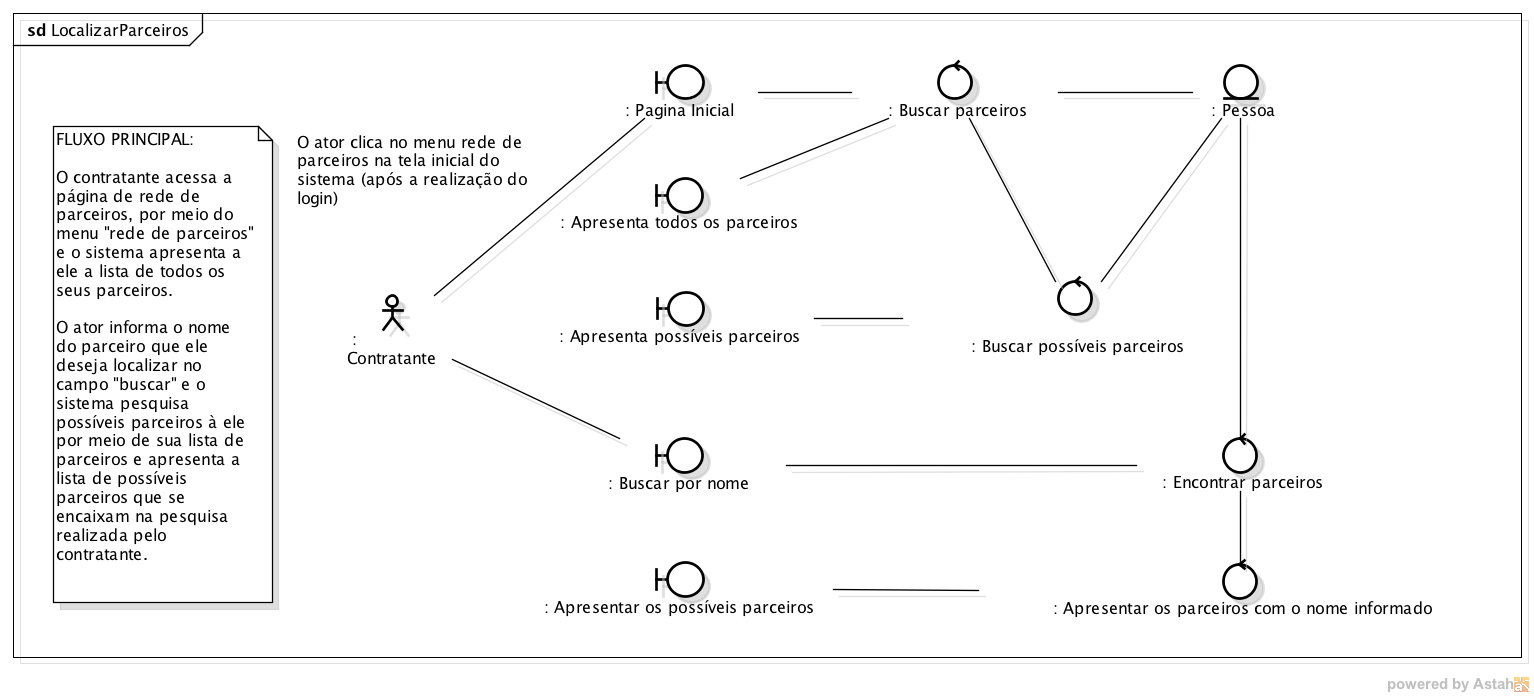
\includegraphics[scale=0.35]{./imagens/apendices/diagrama-robustez-localizar-parceiros.png}}
	\caption[Diagrama de robustez do caso de uso ''Localizar parceiros'']
	{Diagrama de robustez do caso de uso ''Localizar parceiros''. \textbf{Fonte:} Elaborado pelos autores.}
	\label{fig:diagrama_robustez_localizar_mao_de_obra}
\end{figure}

Em paralelo, foi atualizado o modelo de domínio, acrescentando os novos atributos identificados na segunda fase, conforme a Figura~\ref{fig:modelo_dominio_atualizado}.

\begin{figure}[h!]
	\centerline{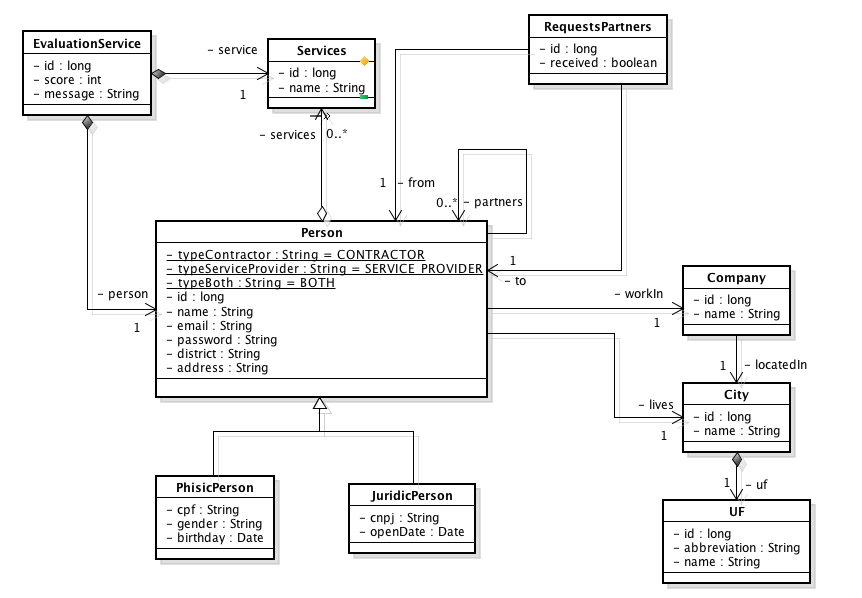
\includegraphics[scale=0.5]{./imagens/modelo-dominio-com-atributos.png}}
	\caption[Modelo de domínio atualizado]
	{Modelo de domínio atualizado. \textbf{Fonte:} Elaborado pelos autores.}
	\label{fig:modelo_dominio_atualizado}
\end{figure}

Com o modelo de domínio atualizado, foi feita a modelagem do banco de dados da aplicação, como apresenta a Figura~\ref{fig:modelo_dados_aplicacao}.

\begin{figure}[h!]
	\centerline{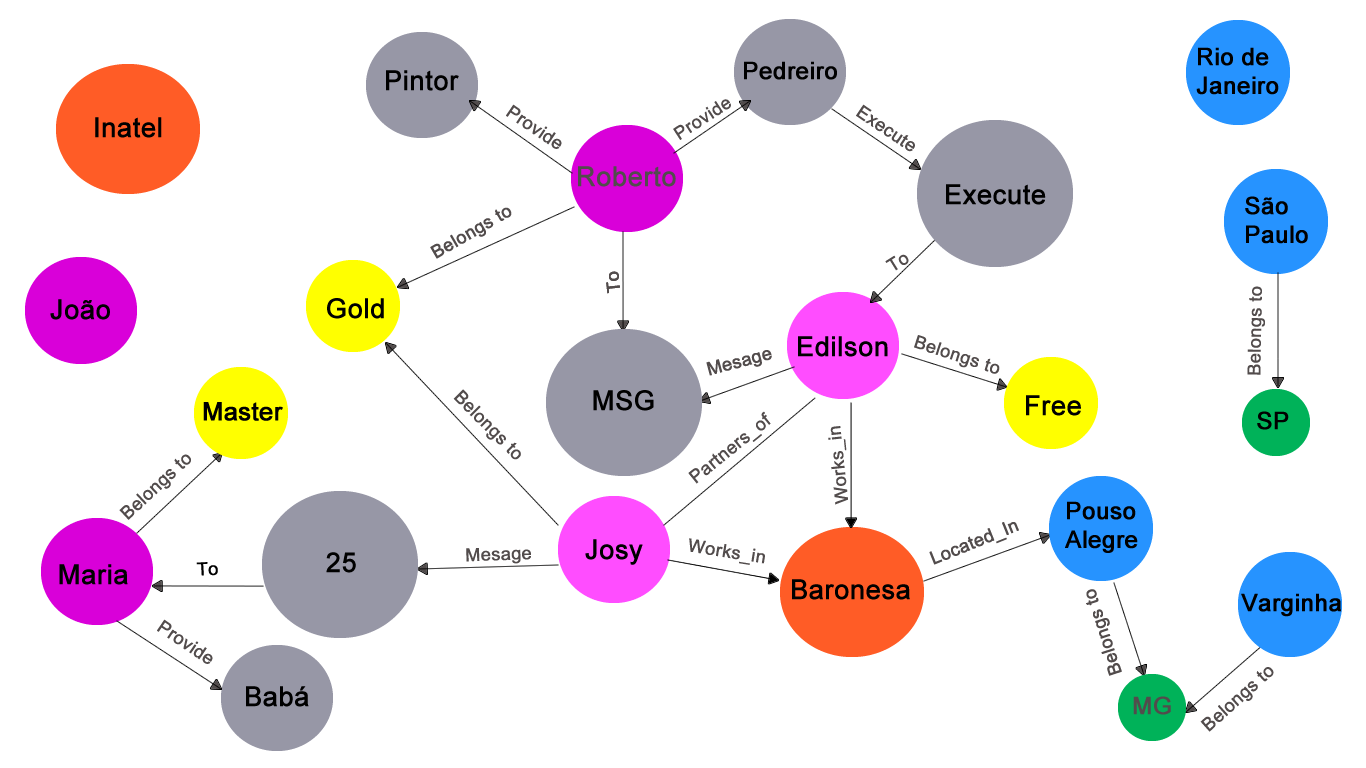
\includegraphics[scale=0.4]{./imagens/structure-all-nodes.png}}
	\caption[Modelo de dados da aplicação]
	{Modelo de dados da aplicação. \textbf{Fonte:} Elaborado pelos autores.}
	\label{fig:modelo_dados_aplicacao}
\end{figure} 

\par Na terceira fase, definida como projeto detalhado, foram criados os diagramas de sequência, tendo como base os casos de uso modelados na fase anterior. Esta fase tem como objetivo detalhar todo o funcionamento do \textit{software}, visando definir a melhor maneira de realizar sua implementação. A Figura~\ref{fig:diagrama_sequencia_localizar_parceiros} apresenta o diagrama de sequência do caso de uso ''Localizar parceiros''.

\newpage
\begin{figure}[h!]
	\centerline{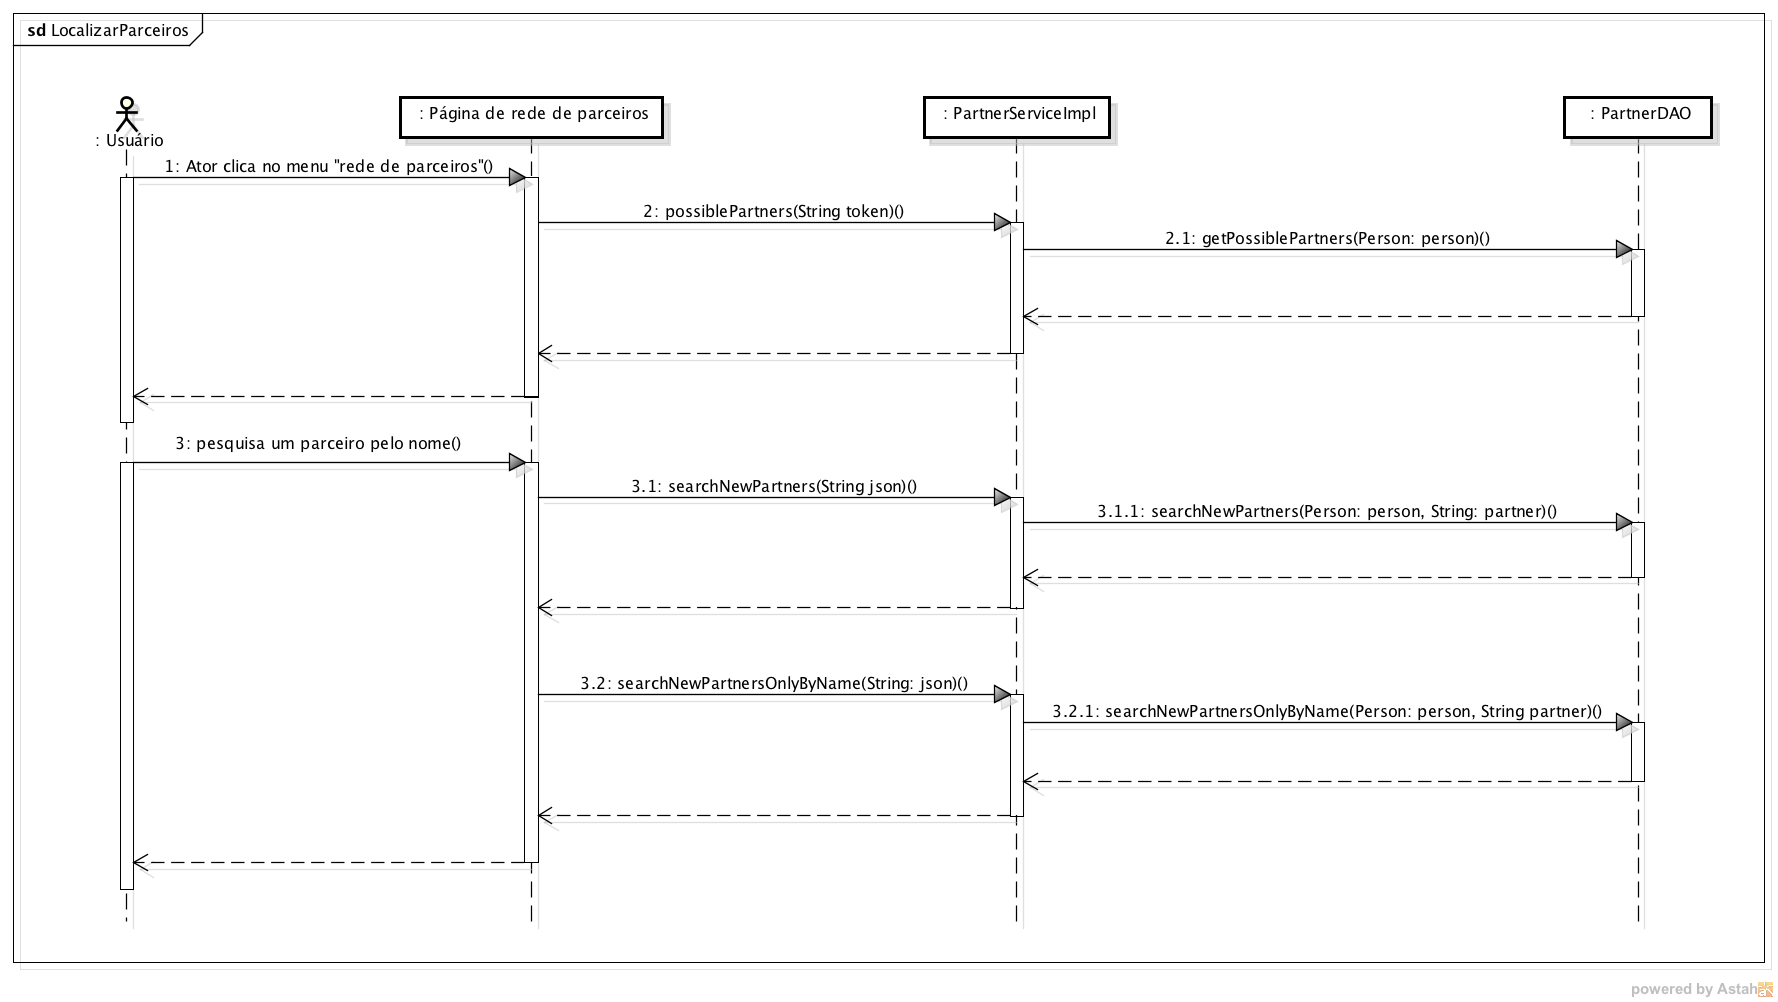
\includegraphics[angle=90,scale=0.4]{./imagens/diagrama-sequencia-localizar-novos-parceiros.png}}
	\caption[Diagrama de sequência do caso de uso ''Localizar parceiros'']
	{Diagrama de sequência do caso de uso ''Localizar parceiros''. \textbf{Fonte:} Elaborado pelos autores.}
	\label{fig:diagrama_sequencia_localizar_parceiros}
\end{figure}

\par Ainda na fase de projeto detalhado, após a modelagem dos diagramas de sequência, as operações encontradas nestes diagramas foram adicionadas ao modelo de domínio, em conjunto com as novas classes identificadas, gerando assim, o digrama de classes como mostra a Figura~\ref{fig:diagrama_classe}.

\begin{figure}[h!]
	\centerline{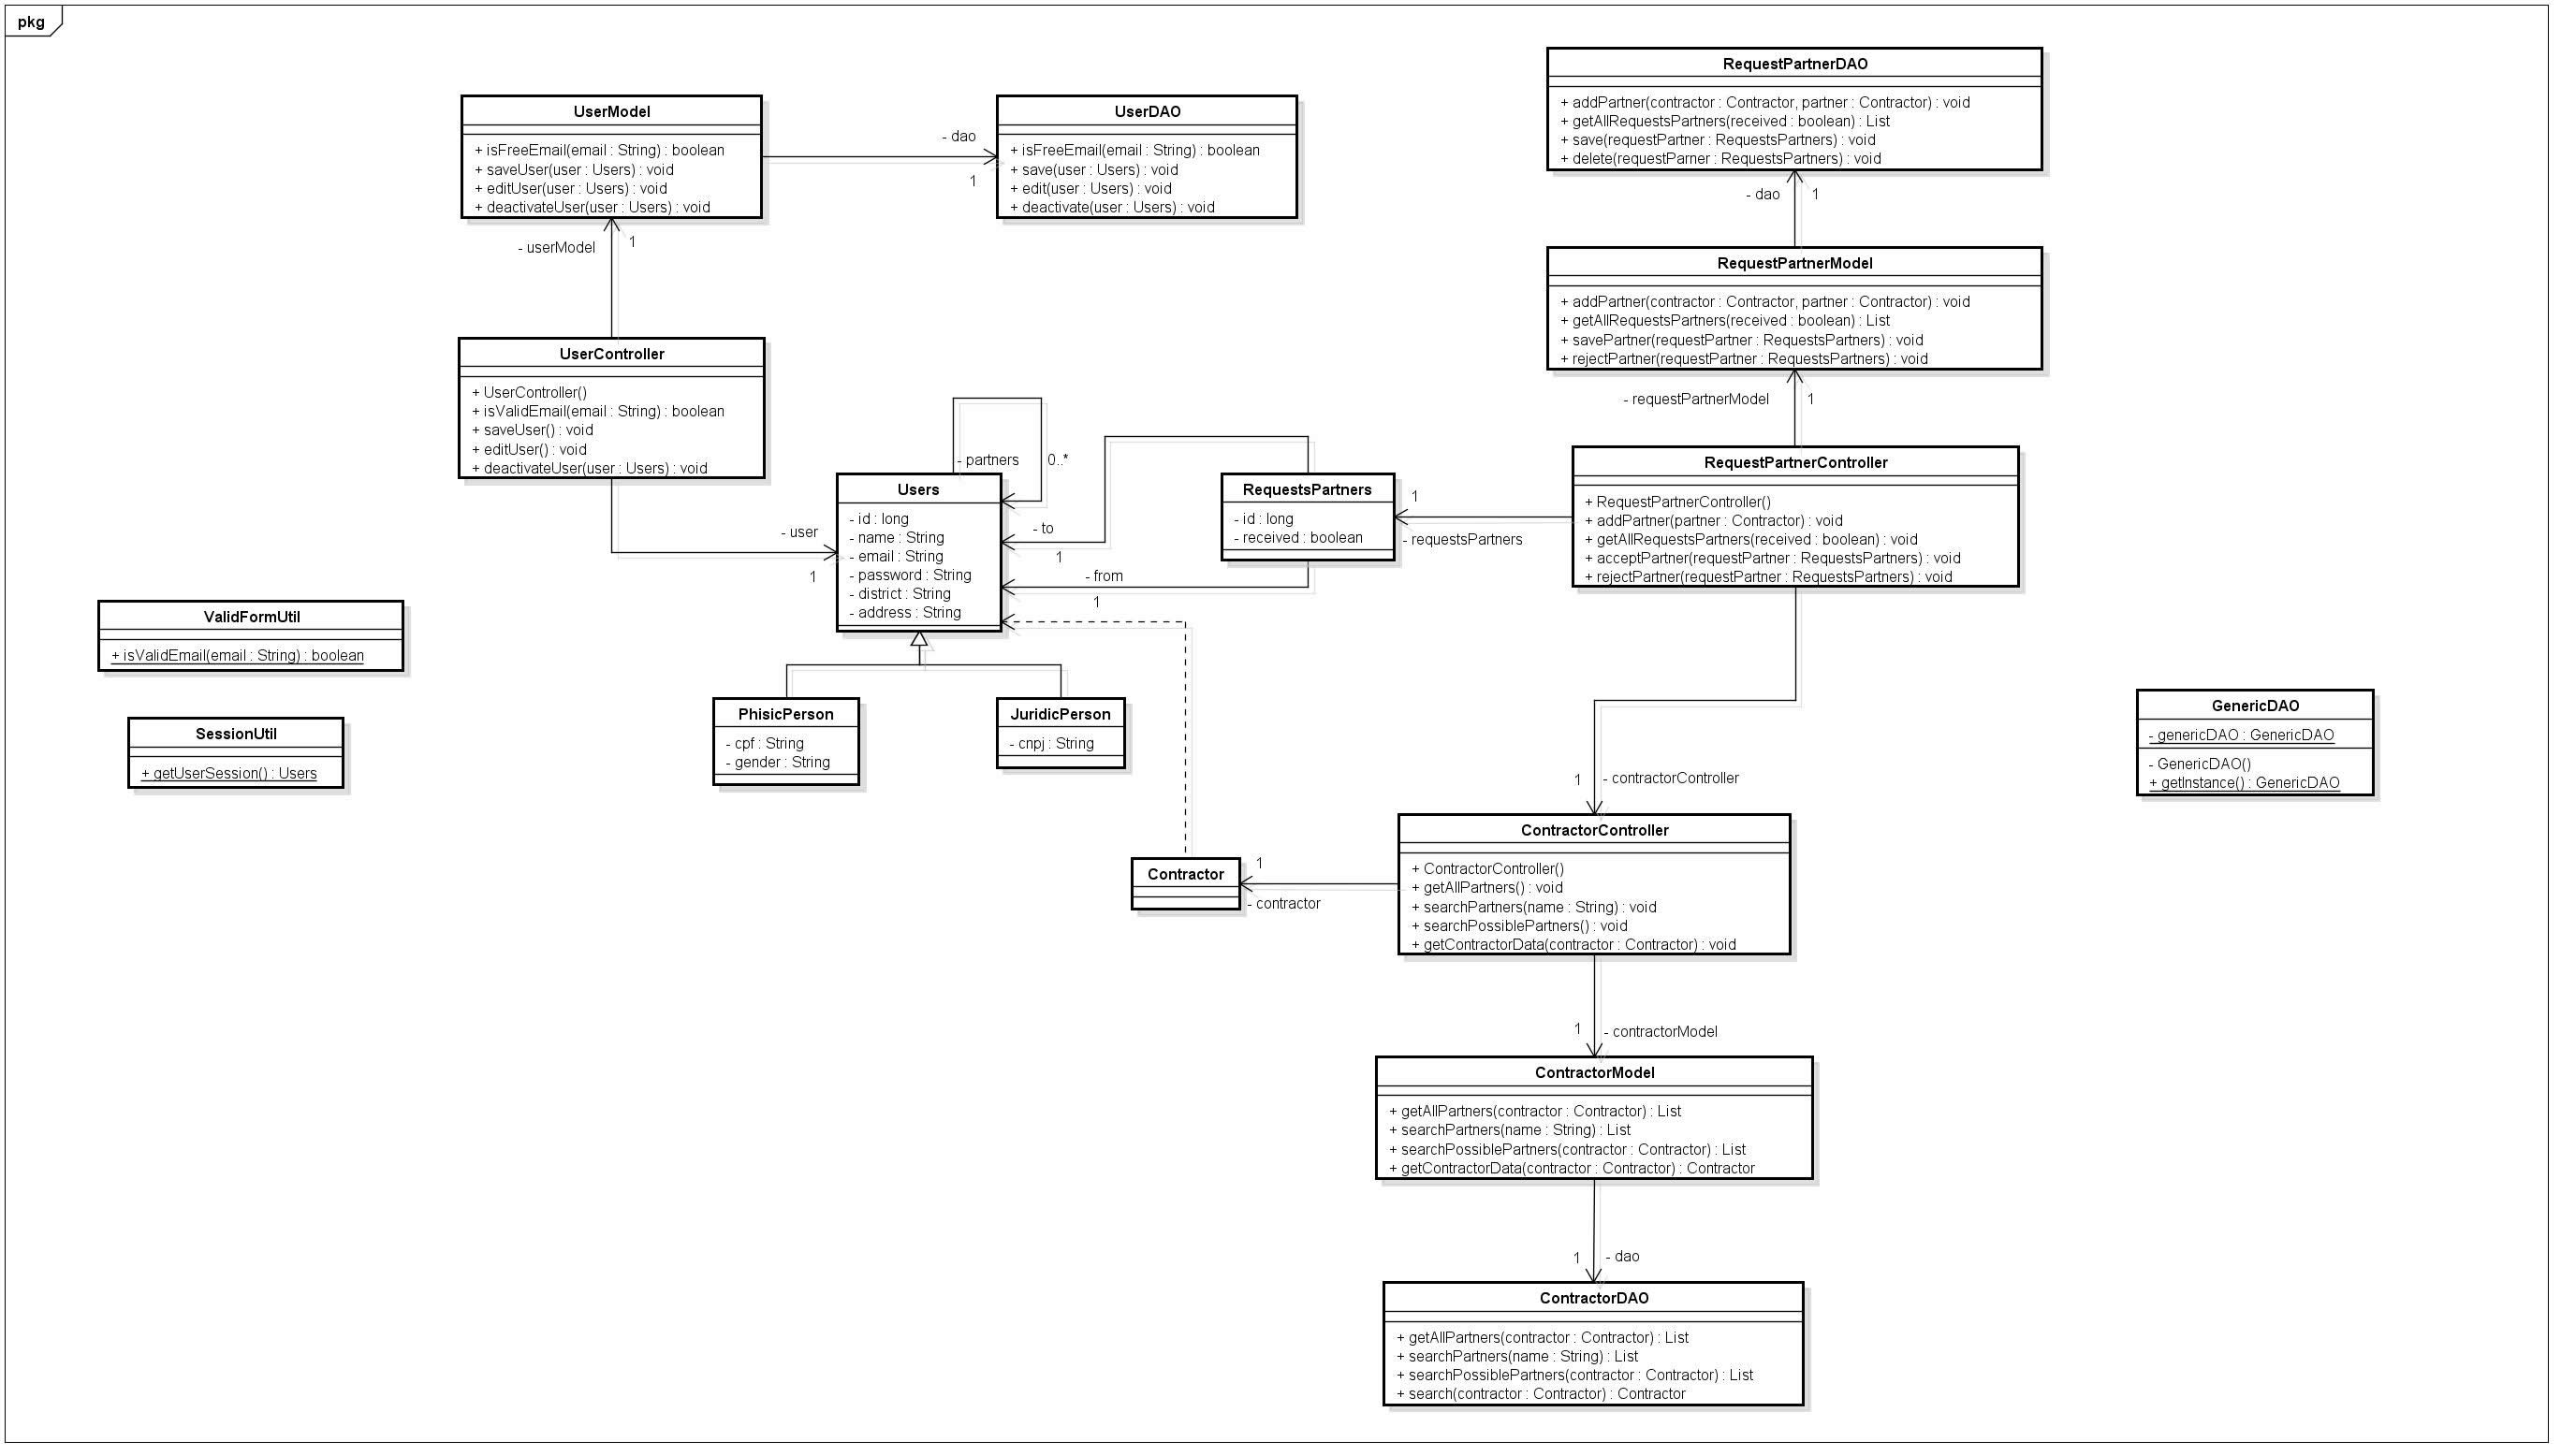
\includegraphics[angle=90,height=0.7\textheight,width=0.7\textwidth]{./imagens/classe.jpg}}
	\caption[Diagrama de classes]
	{Diagrama de classes \textbf{Fonte:} Elaborado pelos autores.}
	\label{fig:diagrama_classe}
\end{figure}

\newpage
\par Na quarta e última fase do ICONIX, denominada implementação, iniciou-se a preparação do ambiente, incluindo a instalação dos \textit{softwares} necessários para o desenvolvimento prático da aplicação. Essa preparação é abordada a seguir.


\section{Teoria dos Grafos}

\par A teoria dos grafos foi criada pelo matemático suiço Leonhard Euler no século XVIII com o propósito de solucionar um antigo problema, conhecido como as 7 pontes de \textit{Königsberg} \cite{harju_graph_theory}.

\par \textit{Königsberg}, atualmente conhecida como \textit{Kaliningrad}, era uma antiga cidade medieval cortada pelo rio \textit{Pregel} dividindo-a em 4 partes interligadas por 7 pontes. Ela era localizada na antiga Prússia, hoje, território Russo. O problema mencionado anteriormente consistia basicamente em atravessar toda a cidade, visitando todas as partes e utilizar todas as pontes desde que não repetisse uma das quatro partes ou uma das 7 pontes. A Figura 2 ilustra o problema mencionado.

% Imagem do problema das 7 pontes da teoria dos grafos
\begin{figure}[h!]
	\centerline{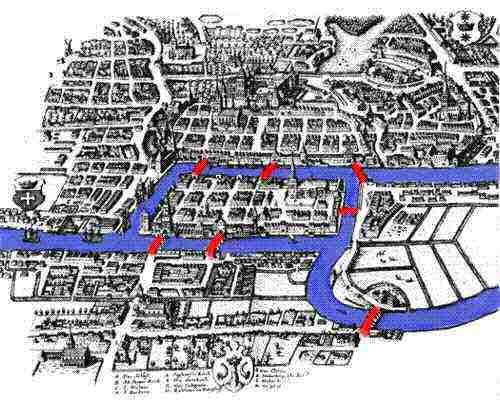
\includegraphics[height=0.26\textheight,width=0.8\textwidth]{./imagens/Konigsberg_7_bridges.jpg}}
	\caption[O problema das 7 pontes de \textit{Königsberg} ]
	{O problema das 7 pontes de \textit{Königsberg}. \textbf{Fonte:} \citeonline{paoletti_seven_bridges_konigsberg}}
	\label{fig:exemplo1}
\end{figure}

\par De acordo com \citeonline{bruggen_learning_neo4j}, para tentar solucionar o problema, Euler utilizou uma abordagem matemática ao contrário dos demais que tentaram utilizar a força bruta para solucionar tal problema, desenhando N números de diferentes possibilidades de rotas. Euler mudou o foco e passou a dar mais atenção ao número de pontes e não as partes da cidade. Por meio desta observação, foi possível perceber que realizar tal tarefa seria impossível, pois de acordo com sua teoria seria necessário possuir no mínimo mais uma ponte, uma vez que, o número de pontes era ímpar, não sendo possível realizar um caminho único e sem repetição. Desta forma, obteve-se a solução para este problema e criou-se o primeiro grafo no mundo.

\par \citeonline[p. 16]{rocha_algoritmos_particionamento_banco_dados_orientado_grafos} afirma que: 

\begin{citacao}
	um \textit{grafo G = (V,E)} consiste em um conjunto finito \textit{V} de vértices e um conjunto finito \textit{E} de arestas onde cada elemento \textit{E} possui um par de vértices que estão conectados entre si e pode ou não possuir um peso \textit{P}.
\end{citacao}

\par Esta é a definição formal de um grafo. A partir desta definição, é possível identificar, no problema mencionado anteriormente, os vértices que neste caso são as pontes e as arestas que por sua vez são as partes da cidade.

\par Segundo \citeonline{bondy_murty_graph_theory_with_applications}, muitas situações do mundo real podem ser descritas através de um conjunto de pontos conectados por linhas formando assim um grafo, como um centro de comunicações e seus \textit{links}, ou as pessoas e seus amigos, ou uma troca de emails entre pessoas, entre outras. Isto é possível pois, de acordo com \citeonline{rocha_algoritmos_particionamento_banco_dados_orientado_grafos}, existem muitos problemas atualmente que podem ser mapeados para uma estrutura genérica possibilitando assim utilizar a teoria de grafos para tentar solucioná-los, tais como: rotas geográficas, redes sociais, entre outros.

%BANCA_QUALIFICACAO. Comentado este parágrafo, porém o mesmo retornará para a banca de qualificação
\par A Figura 3 demostra de maneira visual um grafo, conforme ideia de \citeonline{bondy_murty_graph_theory_with_applications}, utilizando como exemplo o seguinte grafo \textit{G} = \{a, b, c, d, e, f, g, h\} e suas respectivas arestas \textit{E}$_g$ = \{(a, b), (a, h), (a, e), (b, f), (c, e), (c, d), (c, g), (d, e), (d, h), (d, g), (f, h)\}, sendo que os vértices serão representados por círculos e as arestas que os interligam por linhas.

%subscrito $_CARCTER_DESEJADO$

% Imagem do grafo simples - VOLTAR NA BANCA DE QUALIFICACAO
\begin{figure}[h!]
	\centerline{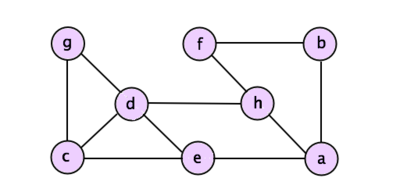
\includegraphics[scale=0.77]{./imagens/simple_graph.png}}
	\caption[Ilustração de uma representação gráfica de um simples grafo]
	{Ilustração de uma representação gráfica de um simples grafo. \textbf{Fonte:} \citeonline{rocha_algoritmos_particionamento_banco_dados_orientado_grafos}}
	\label{fig:exemplo1}
\end{figure}

%BANCA_QUALIFICACAO. Comentado este parágrafo, porém o mesmo retornará para a banca de qualificação
\par \citeonline{ruohonen_graph_theory} afirma que os grafos podem ser gerados com a possibilidade de permitir \textit{loops}\footnotemark[4] e arestas paralelas ou multiplas entre os vértices, obtendo um \textit{multigraph}. A Figura 4 ilustra um simples \textit{multigraph}.

\footnotetext[4]{\textit{loops} - Uma aresta que interliga o mesmo vértice.}

% Imagem de um multigraph - VOLTAR NA BANCA DE QUALIFICACAO
\begin{figure}[h!]
	\centerline{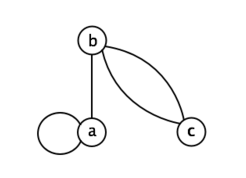
\includegraphics[scale=0.9]{./imagens/multigraph_example.png}}
	\caption[Ilustração de uma representação gráfica de um \textit{multigraph}]
	{Ilustração de uma representação gráfica de um \textit{multigraph}. \textbf{Fonte:} Adaptado de \citeonline{harju_graph_theory}}
	\label{fig:exemplo1}
\end{figure}

\newpage

%BANCA_QUALIFICACAO. Comentado este parágrafo, porém o mesmo retornará para a banca de qualificação
\par Para \citeonline{harju_graph_theory}, os grafos podem ser direcionados (\textit{dígrafo}) ou não direcionados. Os  direcionados são aqueles cujos vértices ligados a uma aresta são ordenados e permitem que uma aresta que conecta os vértices \textit{x} e \textit{y} seja representada apenas de uma forma, sendo ela \{x, y\} ou \{y, x\}, ao contrário dos não direcionados que, para este mesmo caso, podem ser representado por ambas as formas \cite{rocha_algoritmos_particionamento_banco_dados_orientado_grafos}. A Figura 5 demonstra um grafo direcionado.

% Imagem de um grafo direcionado - VOLTAR NA BANCA DE QUALIFICACAO
\begin{figure}[h!]
	\centerline{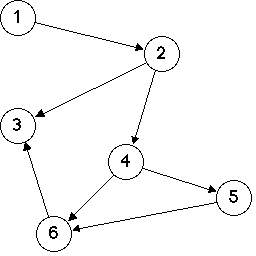
\includegraphics[scale=0.6]{./imagens/simple_digraph_graph.png}}
	\caption[Imagem de uma representação gráfica de um grafo direcionado]
	{Imagem de uma representação gráfica de um grafo direcionado. \textbf{Fonte:} \citeonline{robert_keller_acylic_graph}}
	\label{fig:exemplo1}
\end{figure}

Segundo \citeonline{harju_graph_theory}, os tipos de grafos são:

\begin{itemize}
	\item \textbf{grafo simples:} são aqueles grafos que não possuem \textit{loops} ou arestas paralelas;
	
	\item \textbf{grafo completo:} são aqueles em que, qualquer par de vértices são adjacentes;
	
	\item \textbf{subgrafos:} são pequenos grafos que em conjunto constituem um grafo maior.
	
	\item \textbf{grafos isomórficos:} dois grafos são isomórficos se, ambos possuírem a mesma estrutura de nós, e relacionamentos, exceto pelos identificadores de cada nó que podem ser diferentes, veja na Figura 6 um exemplo de dois grafos isomórficos \cite{harju_graph_theory}.
	
	\begin{figure}[h!]
		\centerline{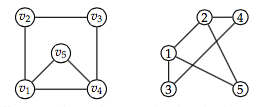
\includegraphics[scale=1]{./imagens/grafos_isomorficos.png}}
		\caption[Imagem de um grafo isomórfico]
		{Imagem de um grafo isomórfico. \textbf{Fonte:} \citeonline{harju_graph_theory}}
		\label{fig:exemplo1}
	\end{figure}
	
	\item \textbf{caminho (travessia):} é uma sequência de vértices \{v1, v2,...,vn\} conectados por meio de arestas. Exemplo: \{e1 = \{v1, v2\}, \{v1, v3\}..., \{vn, vm\}\};

	\item \textbf{grafo conexo:} são aqueles que, para qualquer par de vértices, há um caminho que os ligam;
	
	\item \textbf{grau do vértice:} é definido pela quantidade de arestas que se conectam ao vértice.
	
\end{itemize}

Para \citeonline{rocha_algoritmos_particionamento_banco_dados_orientado_grafos} existem várias formas de se representar um grafo computacionalmente utilizando diferentes estruturas de dados. Entretanto, a mais utilizada e simples é a matriz adjacência.

Uma matriz adjacência consiste em uma matriz contendo o mesmo número de linhas e colunas (\textit{n x n}). Veja na Figura 7 um exemplo de representação de um grafo utilizando esta estrutura.

\begin{figure}[h!]
	\centerline{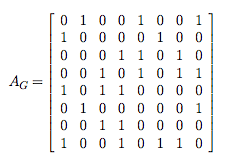
\includegraphics[scale=0.7]{./imagens/matriz_adjacencia.png}}
	\caption[Grafo representado por meio de uma matriz adjacência]
	{Grafo representado por meio de uma matriz adjacência. \textbf{Fonte:} \citeonline{rocha_algoritmos_particionamento_banco_dados_orientado_grafos}}
	\label{fig:exemplo1}
\end{figure}

Na Figura 7, as posições da matriz cujo o valor é igual a 1, definem que há uma aresta conectando os vértices, tornando-os assim, adjacentes. Caso o valor seja 0, os vértices não estão conectados entre si no grafo e, portanto, não são vértices adjacentes.

\par Este conteúdo teórico foi escolhido para ser utilizado neste trabalho pois este visa equacionar o problema relacionado à busca por mão de obra, através do modelo utilizado pelas redes sociais. Isto é possível pois, como mencionado anteriormente por meio desta teoria, é possível descrever várias situações do mundo real e como ela é muito bem aplicada à redes sociais, inclusive grandes empresas desta área já a utilizam. Devido a esses motivos, a teoria dos grafos foi utilizada para auxiliar no desenvolvimento deste trabalho.



\section{Tecnologias}

\par Nesta seção serão abordadas as linguagens de programação e as tecnologias que serão utilizadas para o desenvolvimento deste trabalho.

\subsection{Banco de dados}

\par A expressão ''Banco de dados'' teve origem a partir do termo inglês \textit{Databanks}, que foi substituído, mais tarde, pela palavra \textit{Databases} (Base de dados)  por possuir um significado mais apropriado \cite {setzer_silva_banco_dados_aprenda_o_que_sao_melhore_conhecimento}.

\par De acordo com \citeonline{date_introducao_sistemas_bancos_dados}, um banco de dados é uma coleção de dados persistentes, usada pelos sistemas de aplicação em uma determinada empresa. Sendo assim, um banco de dados é um local onde são armazenados os dados necessários para manter as atividades de determinadas organizações.

\par Um banco de dados possui, implicitamente, as seguintes propriedades: representa aspectos do mundo real; é uma coleção lógica de dados que possuem um sentido próprio e armazena dados para atender uma necessidade específica. O tamanho do banco de dados pode ser variável, desde que ele atenda às necessidades dos interessados em seu conteúdo \cite{elmasri_navathe_sistemas_banco_dados}.

\subsubsection{Tipos de bancos de dados}

\par A escolha do banco de dados que será utilizado em um projeto é uma decisão importante e que deve ser tomada na fase de planejamento, pois determina características da futura aplicação, como a integridade dos dados, o tratamento de acesso de usuários, a forma de realizar uma consulta, o desempenho. Portanto, essa decisão deve ser bem analisada, levando em consideração o tipo de software e no ambiente de produção que será utilizado.

\par A seguir, são demonstrados os principais modelos de banco de dados, abordando suas características.

\subsection{Banco de dados relacionais}

\par O modelo de banco de dados relacional foi introduzido em 1970, por Edgar Frank Codd, em uma publicação com o título: “A relational model of data for large shared data banks”, na revista \textit{Association for Computing Machinery} (ACM). Essa publicação demonstrou como tabelas podem ser usadas para representar objetos do mundo real e como os dados podem ser armazenados para os objetos. Neste conceito, a integridade dos dados foi levada mais a sério do que em qualquer modelo de banco de dados antes visto. A partir desta publicação, surgiram muitos bancos de dados que passaram a utilizar este conceito e se tornaram muito utilizados no desenvolvimento de aplicações
\cite{matthew_stones_beginning_databases_with_postgresql}.

\par Segundo \citeonline{matthew_stones_beginning_databases_with_postgresql}, o conceito é baseado na teoria reacional da matemática e por isso há uma grande flexibilidade para o acesso e a manipulação de dados que são gravados no banco de dados. Utilizam-se técnicas simples, como normalização na modelagem do banco de dados, criando várias tabelas relacionadas, que servem como base para consultas usando uma linguagem de consulta quase padronizada, a \textit{Structured Query Language} – SQL\footnotemark[5].

\footnotetext[5]{SQL: \textit{Structured Query Language} - Linguagem para consultas e alterações em bancos de dados.}

% Pode voltar mais a frente no TCC quando for necessário aumentar esta parte
%\par Ainda segundo \citeonline{matthew_stones_beginning_databases_with_postgresql}, um banco de dados relacional contém relações (tabelas) com atributos (colunas) e tuplas (linhas). Todo atributo possui um tipo de dado predefinido, uma tupla representa um conjunto de dados contendo um valor para cada atributo da linha e as tabelas são relacionadas através de chaves.

\par A utilização de banco de dados relacionais geraram a necessidade de dividir os dados agregados utilizados na aplicação em várias relações conforme as regras da normalização. Para recuperar o mesmo dado agregado são necessárias consultas utilizando \textit{joins}\footnotemark[6], uma operação que, dependendo do tamanho das relações e da quantidade de dados, pode não ser tão eficiente. Nos casos em que se precisa obter uma resposta rápida de um sistema, isso se torna uma desvantagem \cite{sadalage_fowler_nosql_distilled_brief_guide}.

\footnotetext[6]{\textit{joins} - função utilizada para realizar a junção entre tabelas, facilitando a busca em bancos de dados relacionais.}

% Pode voltar mais a frente no TCC quando for necessário aumentar esta parte
%\par A figura 6 ilustra bem esta situação de divisão de um agregado e as suas relações resultantes.

% Imagem do exemplo de join - PODE VOLTAR MAIS TARDE NO TCC (Confirmar com o Márcio)
%\begin{figure}[h!]
	%\centerline{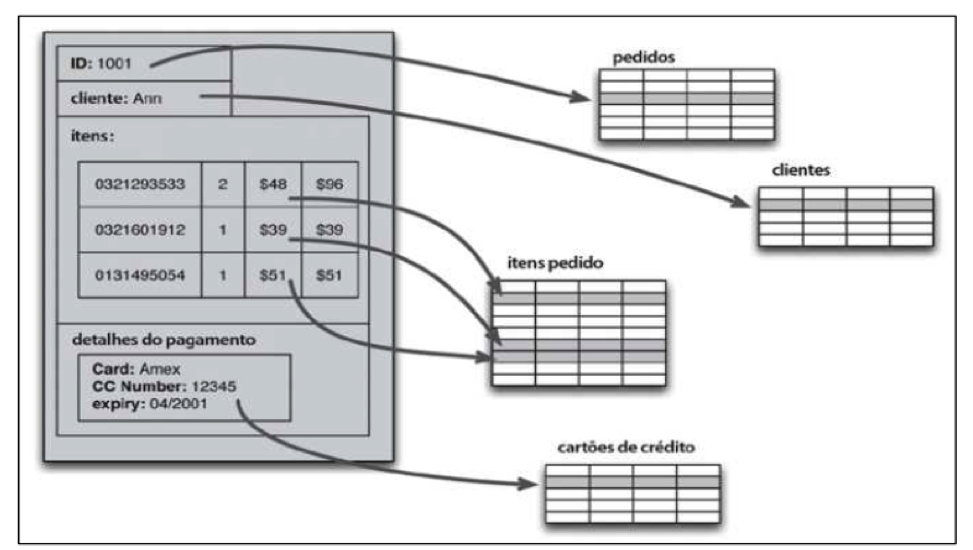
\includegraphics[scale=0.8]{./imagens/example_joins_sadalage.png}}
	%\caption[Agregado no UI é conjunto de várias tuplas de várias tabelas]
	%{Agregado no UI é conjunto de várias tuplas de várias tabelas. \textbf{Fonte:} \citeonline[p. 29]{sadalage_fowler_nosql_distilled_brief_guide}}
	%\label{fig:exemplo1}
%\end{figure}

\par Este foi um dos fatores determinantes que motivaram a criação de novas tecnologias, a fim de sanar o problema mencionado acima. A partir desta motivação, foram desenvolvidos novos modelos de banco de dados, que serão apresentados a seguir.


\subsection{Banco de dados NoSQL}

\par A expressão NoSQL é um termo não definido claramente. Ela foi ouvida pela primeira vez em 1998 como um nome para o banco de dados relacional de Carlo Strozzi, que assim o nomeou por não fornecer uma SQL-API. O mesmo termo foi usado como nome do evento NoSQL Meetup em 2009, que teve como objetivo a discussão sobre sistemas de bancos de dados distribuídos.

\par Devido a explosão de conteúdos na \textit{web} no início do século XXI, houve-se a necessidade de substituir os bancos de dados relacionais por bancos que oferececem maior capacidade de otimização e performance, a fim de suportar o grande volume de informações eminentes a esta mudança \cite{bruggen_learning_neo4j}.

\par \citeonline[p. 27]{rocha_algoritmos_particionamento_banco_dados_orientado_grafos} afirma que NoSQL é "um acrônimo para Not only SQL, indicando que esses bancos não usam somente o recurso de Structured Query Language (SQL), mas outros recursos que auxiliam no armazenamento e na busca de dados em um banco  não relacional".

\par Segundo \citeonline{bruggen_learning_neo4j}, os banco de dados NoSQL podem ser categorizados de 4 maneiras diferentes, são elas: \textit{Key-Value stores}\footnotemark[6], \textit{Column-Family stores}\footnotemark[7], \textit{Document stores}\footnotemark[8] e \textit{Graph Databases}\footnotemark[9].

\footnotetext[6]{\textit{Key-Value stores} - armazenamento por um par de chave e valor.}

\footnotetext[7]{\textit{Column-Family stores} - armazenamento por colunas e linhas.}

\footnotetext[8]{\textit{Document stores} - armazenamento em arquivos.}

\footnotetext[9]{\textit{Graph Databases} - banco de dados orientado a grafo.}
%\begin{itemize}
%\item \textit{Key-Value stores};
%\item \textit{Column-Family stores};
%\item \textit{Document stores};
%\item \textit{Graph Databases}.
%\end{itemize}

\par De acordo com \citeonline{bruggen_learning_neo4j}, o banco de dados orientado a grafo (\textit{graph database}) pertence a categoria NoSQL, contudo, ele possui particularidades que o torna muito diferente dos demais tipos de bancos de dados NoSQL. A seguir, será descrito com maiores detalhes o banco de dados orientado a grafos Neo4j.


\subsection{Neo4j}

\par O Neo4j foi criado no início do século XXI por desenvolvedores que queriam resolver um problema em uma empresa de mídias. Porém, eles não obtiveram êxito ao tentar resolver tal problema utilizando as tecnologias tradicionais, portanto, decidiram arriscar e criar algo novo. A princípio, o Neo4j não era um sistema de gerenciamento de banco de dados orientado a grafos como é conhecido nos dias atuais. Ele era mais parecido com uma \textit{graph library} (biblioteca de grafo) em que as pessoas poderiam usar em seus projetos \cite{bruggen_learning_neo4j}.

\par De acordo com \citeonline{bruggen_learning_neo4j}, inicialmente ele foi desenvolvido para ser utilizado em conjunto com alguns bancos de dados relacionais como MySQL e outros, com a intenção de criar uma camada de abstração dos dados em grafos. Mas com o passar dos anos, os desenvolvedores decidiram tirar o Neo4j da estrutura dos bancos relacionais e criar sua própria estrutura de armazenamento em grafos.

\par O Neo4j, como vários outros, também é um projeto de sistema de gerenciamento de banco de dados NoSQL de código fonte aberto.

\par Segundo \citeonline{robinson_webber_eifrem_graph_databases}, os bancos de dados orientados a grafos possuem como diferencial a sua performance, agilidade e flexibilidade. Entretanto, a performance é o que mais se destaca entre eles, pois, a maneira como eles armazenam e realizam buscas no banco de dados é diferente dos bancos de dados convencionais. Primeiramente, esse tipo de banco de dados não utiliza tabela; ele armazena os dados em vértices e arestas. Isso permite realizar buscas extremamente velozes através de \textit{traversals} (travessias), uma vez que estas implementam algoritmos para otimizar tais funcionalidades, evitando assim o uso de \textit{joins} complexos, tornando-o tão veloz.

\par \citeonline[p. 2]{neo4j_team_manual} afirma que:

\begin{citacao}
	\textit{A single server instance can handle a graph of billions of nodes and relationships. When data throughput is insufficient, the graph database can be distributed among multiple servers in a high availability configuration.}\footnotemark[11]
\end{citacao}

\footnotetext[11]{Um único servidor pode manipular um grafo de bilhões de nós e relacionamentos. Quando a taxa de transferência de dados é insuficiente, o banco de dados orientado a grafo pode ser distribuído entre vários servidores mantendo a mesma velocidade de processamento.}

\par Com estas informações, é possível mensurar o quanto o Neo4j pode ser rápido e robusto, sendo possível, até mesmo distribuí-lo a fim de obter uma melhor configuração, organização e facilidade de manutenção.

%BANCA_QUALIFICACAO. Comentado este parágrafo, porém o mesmo retornará para a banca de qualificação
\par Segundo \citeonline{neo4j_team_manual}, o banco de dados Neo4j é composto por nós (vértices), relacionamentos (arestas) e propriedades. Os relacionamentos são responsáveis por organizar os nós e ambos podem possuir seus atributos. É possível realizar as buscas e/ou alterações no Neo4j de duas formas diferentes. Sendo a primeira através da API \textit{Cypher Query Language}, que é uma \textit{query language} para banco de dados orientado a grafos muito próxima da linguagem humana, cuja descrição completa será apresentada a seguir. A segunda é o \textit{framework\footnotemark[12] Traversal} que utiliza a API \textit{Cypher} internamente para navegar pelo grafo.

\footnotetext[12]{\textit{Framework} - Abstração que une códigos comuns entre vários projetos de software, a fim de obter uma funcionalidade genérica.}


\citeonline{rocha_algoritmos_particionamento_banco_dados_orientado_grafos} afirma que o Neo4j permite criar mais de um relacionamento entre o mesmo par de vértices, desde que estes sejam de tipos distintos. Isso possibilita navegar pelos vértices do grafo de forma mais rápida devido a esses diferentes tipos de arestas, o que torna possível implementar o algoritmo de busca desejado. A Figura~\ref{fig:grafo_simples_neo4j} exemplifica um simples grafo utilizando um banco de dados Neo4j.


\begin{figure}[h!]
	\centerline{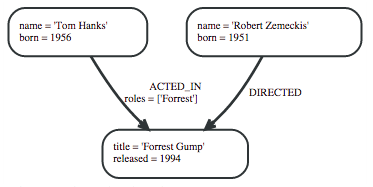
\includegraphics[scale=0.8]{./imagens/simple_graph_neo4j.png}}
	\caption[Exemplo simples de um grafo no Neo4j]
	{Exemplo simples de um grafo no Neo4j. \textbf{Fonte:} \citeonline{neo4j_team_manual}}
	\label{fig:grafo_simples_neo4j}
\end{figure}

\newpage
%BANCA_QUALIFICACAO. Comentado este parágrafo, porém o mesmo retornará para a banca de qualificação
\par Há duas formas de executar o Neo4j, segundo \citeonline{robinson_webber_eifrem_graph_databases}. A primeira é conhecida como \textit{Server} e a segunda \textit{Embedded}. O modo \textit{Server} é utilizado principalmente em \textit{web-service} em conjunto com a API REST, este será aplicado neste trabalho. Já no modo \textit{Embedded} o banco de dados é executado embarcado à aplicação Java.

%BANCA_QUALIFICACAO. Comentado este parágrafo, porém o mesmo retornará para a banca de qualificação
\par Conforme \citeonline{neo4j_team_manual}, o Neo4j possui suporte as transações ACID (com atomicidade, consistência, isolamento e durabilidade).

O Neo4j é distribuído em duas versões sendo elas a \textit{Entreprise} e a \textit{Community}. A primeira possui um tempo de avaliação de 30 dias e após esse tempo, é necessário comprar uma licença para continuar a utilizá-lo. Como diferencial essa versão possui ferramentas para o gerenciamento do banco de dados, incluindo melhorias relacionadas à escalabilidade. A segunda versão é disponibilizada gratuitamente sem data limite de expiração, contudo, ela não possui os recursos mencionados anteriormente que estão presentes na versão \textit{Enterprise}, mas é muito utilizada para fins didáticos e para pequenos projetos, aplicando-se perfeitamente a este projeto \cite{neo4j_team_manual}.

\par Por ser um banco de dados orientado a grafo bastante robusto, seguro e possuir uma documentação de fácil entendimento, além, é claro, de possuir um baixo custo de implantação devido a sua licença \textit{open source}, esse banco de dados foi escolhido para ser utilizado neste trabalho.


\subsection{\textit{Cypher Query Language}}

\par O \textit{Cypher Query Language} é uma linguagem para consultas em banco de dados orientado a grafo específica para o banco Neo4j. Ela foi criada devido à necessidade de manipular os dados e realizar buscas em grafos de uma forma mais simples, uma vez que, não é necessário escrever \textit{traversals} (\textit{travessias}) para navegar pelo grafo \cite{neo4j_team_manual}.


\par \citeonline{robinson_webber_eifrem_graph_databases}, afirmam que, o \textit{Cypher} foi desenvolvido para ser uma \textit{query language} que utiliza uma linguagem formal, permitindo a um ser humano entendê-la. Desta forma, qualquer pessoa envolvida no projeto é capaz de compreender as consultas realizadas no banco de dados. 

%BANCA_QUALIFICACAO. Comentado este parágrafo, porém o mesmo retornará para a banca de qualificação
\par Segundo \citeonline{neo4j_team_manual}, o \textit{Cypher} foi inspirado em uma série de abordagens e construído sob algumas práticas já estabelecidas, inclusive a SQL. Por este motivo, é possível notar que ele utiliza algumas palavras reservadas que são comuns na SQL como \textit{WHERE} e \textit{ORDER BY}.

%BANCA_QUALIFICACAO. Comentado este parágrafo, porém o mesmo retornará para a banca de qualificação
\par De acordo com \citeonline{neo4j_team_manual}, o \textit{Cypher} é composto por algumas cláusulas, dentre elas, se destacam:

%%BANCA_QUALIFICACAO. Comentado estes itens, porém os mesmos retornarão para a banca de qualificação
\begin{itemize}
	\item \textit{START}: Define um ponto inicial para a busca, este ponto pode ser um relacionamento ou um nó.
	\item \textit{MATCH}: Define o padrão de correspondência entre os nós. Para identificar um nó é necessário incluí-lo entre um par de parenteses, e os relacionamentos são identificados um hífen e um sinal de maior ou menor.
	\item \textit{CREATE}: Utilizado para criar nós e relacionamentos no grafo.
	\item \textit{WHERE}: Define um critério de busca.
	\item \textit{RETURN}: Define quais nós, relacionamentos e propriedades de ambos devem ser retornados da \textit{query} realizada. 
	\item \textit{SET}: Utilizado para editar as propriedades de um nó ou de um relacionamento.
	\item \textit{UNION}: Possibilita juntar o resultado de duas ou mais consultas.
	\item \textit{FOREACH}: Realiza uma ação de atualização para cada elemento na lista.
\end{itemize} 

\par Outras \textit{Query Languages} existem, inclusive com suporte ao Neo4j, porém devido as vantagens apresentadas acima, somada ao fato que ele possui uma curva de aprendizagem menor e é excelente para lhe oferecer uma base a respeito de grafos,  este \textit{framework} será utilizado para realizar as tarefas de manipulação dos dados no banco de dados.


\subsection{Java}

\par Segundo \citeonline{schildt_java_complete_reference}, a primeira versão da linguagem Java foi criada por James Gosling, Patrick Naughton, Chris Warth, Ed Frank e Mike Sheridan na \textit{Sun Microsystems} em 1991 e denominada "Oak" cujo seu principal foco era a interatividade com a TV. Mais tarde, em 1995, a \textit{Sun Mycrosystems} renomeia esta linguagem e anuncia publicamente a tecnologia Java, focando nas aplicações \textit{web}, que em pouco tempo e devido à grande ascensão da internet, cresceu e se mantém em constante evolução até os dias atuais.

\par De acordo com a \citeonline{oracle_about_java_technology}, a tecnologia Java não é apenas uma linguagem, mas também uma plataforma, que teve como modelo uma outra linguagem, o C++ que, por sua vez foi derivada da linguagem C. O C++ e o Java possuem em comum o conceito de orientação a objetos. O que permite a esta linguagem utilizar recursos como: generalização (herança), implementação, polimorfismo, entre outras. Tais funcionalidades permitem ao desenvolvedor escrever códigos reutilizáveis, a fim de facilitar o desenvolvimento do projeto.

\par Para \citeonline{schildt_java_complete_reference}, o paradigma de orientação a objetos foi criado devido às limitações que o conceito estrutural apresentava quando era utilizado em projetos de grande porte, dificultando o desenvolvimento e manutenção dos mesmos. Este paradigma possibilita ao desenvolvedor aproximar o mundo real ao desenvolvimento de \textit{software}, deixando os objetos do mundo real semelhantes a seus respectivos objetos da computação, possibilitando ao desenvolvedor modelar seus objetos de acordo com suas necessidades \cite{tcc_univas_faria_aspectj_programacao_orientada_aspecto_java}.

Segundo \citeonline{schildt_java_complete_reference}, o recurso denominado generalização (herança) permite ao desenvolvedor criar uma classificação hierárquica de classes. Além disso, é possível escrever uma classe genérica contendo comportamentos comum, e as demais classes, cujo tais comportamentos também serão aplicados a ela, somente precisa generalizar esta classe.

O polimorfismo se refere ao princípio da biologia em que um organismo pode ter diferentes formas ou estados. Este mesmo princípio, também pode ser aplicado à programação orientada a objeto. Desta forma, é possível definir comportamentos que serão compartilhadas entre as classes e suas respectivas sub classes, além de comportamentos próprios cujo apenas as sub classes possuem. Com isto, o comportamento pode ser diferente de acordo com a forma e/ou o estado do objeto \cite{polymorphism_oracle}.

\par Retomando a ideia da \citeonline{oracle_about_java_technology}, uma das vantagens da tecnologia Java sob as demais é o fato de ela ser multiplataforma, possibilitando ao desenvolvedor escrever o código apenas uma vez e este, ser executado em qualquer plataforma inclusive em hardwares com menor desempenho. Isto é possível, pois, para executar um programa em Java é necessário possuir uma \textit{Java Virtual Machine} - JVM\footnotemark[12] - instalada no computador. A JVM compreende e executa apenas \textit{bytecodes}\footnotemark[13] e estes por sua vez são obtidos através do processo de compilação do código escrito em Java.

%Nota a respeito da sigla JVM
\footnotetext[12]{JVM: \textit{Java Virtual Machine} - Máquina virtual utilizada pela linguagem Java para execução e compilação de \textit{softwares} desenvolvidos em Java.}

%Nota a respeito de bytecodes
\footnotetext[13]{\textit{Bytecode} é o código interpretado pela JVM. Ele é obtido por meio do processo de compilação de um programa java como mencionado anteriormente.}

\par Todo programa que utiliza Java necessita passar por algumas etapas essenciais. Conforme ilustrado na figura 9, o código é escrito em arquivo de texto com extensão \texttt{.java}, após isto ele será compilado e convertido para um arquivo com extensão \texttt{.class}, cujo o texto é transformado em \textit{bytecodes}. Este arquivo com extensão \texttt{.class} é interpretado pela JVM que é responsável por executar todo o código do programa.

\newpage
% Imagem do Processo de compilação do Java
\begin{figure}[h!]
	\centerline{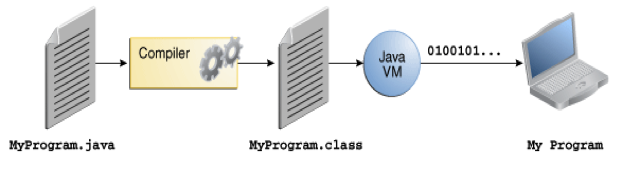
\includegraphics[scale=1]{./imagens/processo_compilacao_java.png}}
	\caption[Uma visão geral do processo de desenvolvimento de software.]
	{Uma visão geral do processo de desenvolvimento de software. \textbf{Fonte:} \citeonline{oracle_about_java_technology}}
	\label{fig:exemplo1}
\end{figure}

\par Por todas as vantagens descritas acima, será empregado o uso desta tecnologia neste projeto.


\subsection{Tomcat 7}

\par O Tomcat é uma aplicação \textit{container}, capaz de hospedar aplicações \textit{web} baseadas em Java. A princípio ele foi criado para executar \textit{servlets}\footnotemark[15] e \textit{JavaServer Pages} - JSP\footnotemark[16]. Inicialmente ele era parte de um sub projeto chamado \textit{Apache-Jakarta}, porém, devido ao seu sucesso ele passou a ser um projeto independente, e hoje, é responsabilidade de um grupo de voluntários da comunidade \textit{open source} do Java \cite{vukotic_goodwill_apache_tomcat_7}.

\footnotetext[15]{\textit{Servlet} - Programa Java executado no servidor, semelhante a um \textit{applet}.}

\footnotetext[16]{JSP: \textit{JavaServer Pages} - Tecnologia utilizada para desenvolver páginas interativas utilizando Java \textit{web}.}

\par Segundo a \citeonline{apache_about_tomcat}, o Tomcat é um software que possui seu código fonte aberto e disponibilizado sob a \textit{Apache License Version 2}. Isto o fez se tornar uma das aplicações \textit{containers} mais utilizadas por desenvolvedores.

\par \textit{Containers} são aplicações que são executadas em servidores e possuem a capacidade de hospedar aplicações desenvolvidas em Java \textit{web}. O servidor ao receber uma requisição do cliente, entrega esta ao \textit{container} no qual é distribuído. O \textit{container}, por sua vez, entrega ao \textit{servlet} as requisições e respostas HTTP\footnotemark[17] e inicia os métodos necessários do \textit{servlet} de acordo com o tipo de requisição realizada pelo cliente \cite{basham_sierra_bates_use_cabeca_servlets_jsp}.

\footnotetext[17]{HTTP: \textit{Hypertext Transfer Protocol} - Protocolo de transferência de dados mais utilizado na rede mundial de computadores.}

%BANCA_QUALIFICACAO. Comentado este parágrafo, porém o mesmo retornará para a banca de qualificação
\par \citeonline{brittain_darwin_apache_tomcat_2nd_edition} afirmam que o Tomcat foi desenvolvido utilizando a linguagem de programação Java, sendo necessário possuir uma versão do \textit{Java Runtime Environment} - JRE\footnotemark[18] - instalada e atualizada para executá-lo.

\footnotetext[18]{JRE: \textit{Java Runtime Environment} - Conjunto de ferramentas necessárias para a execução de aplicações desenvolvidas na linguagem Java.}
%BANCA_QUALIFICACAO. Comentado este parágrafo, porém o mesmo retornará para a banca de qualificação
\par De acordo com  \citeonline{laurie_laurie_apache_the_definitive_guide}, o Tomcat é responsável por realizar a comunicação entre a aplicação e o servidor Apache\footnotemark[19] por meio do uso de \textit{sockets}.

\footnotetext[19]{Apache - Servidor cujo aplicação Tomcat é executada.}

\par Assim como outros \textit{containers}, \citeonline{basham_sierra_bates_use_cabeca_servlets_jsp} afirmam que o Tomcat oferece gerenciamento de conexões \textit{sockets}, suporta \textit{multithreads}, ou seja, ele cria uma nova \textit{thread} para cada requisição realizada pelo cliente e gerencia o acesso aos recursos do servidor, além de outras tarefas.

\par O Tomcat, em especial, foi escolhido para ser utilizado neste trabalho, pois o objetivo é desenvolver uma aplicação \textit{web} e para hospedá-la em um servidor, uma aplicação \textit{container} se faz necessária. Por este motivo, e somado a sua facilidade de configuração, além das vantagens acima descritas tal decisão foi tomada.


\subsection{JavaServer Faces}

\par Segundo \citeonline{faria_java_ee_7_jsf_primefaces_cdi}, a tecnologia \textit{JavaServer Faces} - JSF\footnotemark[21] - foi definida pelo JCP (\textit{Java Community Process}), tornando-a um padrão de desenvolvimento, facilitando assim o trabalho dos desenvolvedores de software.

\footnotetext[21]{JSF: \textit{JavaServer Faces} - Framework que permite desenvolver páginas \textit{web} para aplicações desenvolvidas em Java.}

\par \citeonline{bergsten_javaserver_faces} afirma que o JSF é um \textit{framework server-side} baseado em componentes \textit{web}, cuja principal função é abstrair os detalhes de manipulação dos eventos e organização dos componentes na página \textit{web}. Por meio dele é possível desenvolver páginas mais sofisticadas de forma simples, abstraindo inclusive, o tratamento de requisições e respostas. Isto permite ao desenvolvedor focar-se no \textit{back-end} da aplicação, ou seja, na lógica, e não se preocupar com detalhes a respeito de requisições e respostas HTTP e como obter as informações recebidas e/ou enviadas através deste protocolo.

\par De acordo com \citeonline{oracle_javaserver_faces_technology_overview}, o JSF é de fácil aprendizado e utilização, pois possui sua arquitetura claramente definida, sendo dividida entre a lógica da aplicação e apresentação. Esta divisão é possível pois ele utiliza o padrão de projeto \textit{Model-View-Controller} - MVC\footnotemark[22] -, tornando-o um importante \textit{framework} para desenvolvimento de aplicações utilizando a plataforma Java \textit{Web} e com alta demanda no mercado.

\footnotetext[23]{MVC: \textit{Model-View-Controller} - \textit{Design pattern}.}

%BANCA_QUALIFICACAO. Comentado este parágrafo, porém o mesmo retornará para a banca de qualificação
\par Segundo \citeonline{gamma_helm_johnson_vlissides_design_patterns_elements_reusable_object_oriented_software}, o padrão de projeto MVC é dividido em três partes. O \textit{Model} é a lógica da aplicação, a \textit{View} é camada de apresentação e por último o \textit{Controller} é responsável por definir a interface entre a lógica e a apresentação. Portanto, todo tipo de requisição ou resposta deve ser obrigatoriamente enviada ao \textit{Controller}, que, por sua vez encaminhará para a camada de visão ou de lógica. A figura 7 demonstra um exemplo do modelo MVC utilizando o JSF.

% Imagem do modelo MVC usando JSF - VOLTAR PARA A BANCA DE QUALIFICACAO
\begin{figure}[h!]
	\centerline{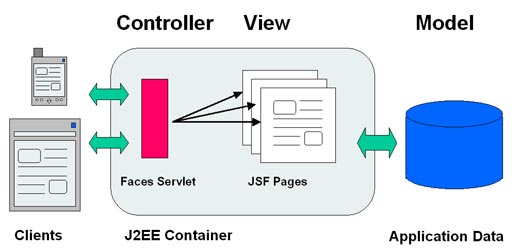
\includegraphics[scale=0.5]{./imagens/jsf_using_mvc.jpg}}
	\caption[Imagem de demonstração do Modelo MVC]
	{Imagem de demonstração do Modelo MVC \textbf{Fonte:} http://www.javabeat.net/jsf-2/}
	\label{fig:exemplo1}
\end{figure}

%BANCA_QUALIFICACAO. Comentado este parágrafo, porém o mesmo retornará para a banca de qualificação
\par Ao utilizar o JSF, toda e qualquer interação que o usuário realizar com a aplicação será executada por um \textit{servlet} chamado \textit{Faces Servlet}. Ela é a responsável por receber tais requisições da camada de visão e redirecioná-las à lógica da aplicação e, posteriormente, enviar a resposta ao usuário \cite{faria_java_ee_7_jsf_primefaces_cdi}.

\par Por possuir as vantagens descritas acima e possuir uma simples configuração, além de ser um \textit{framework cross-browser\footnotemark[19]}, este \textit{framework} foi escolhido para auxiliar no desenvolvimento das páginas \textit{web} deste projeto.

\footnotetext[23]{\textit{Cross-Browser} - Compatibilidade com todos os tipos de dispositivos e navegadores}


\subsection{Primefaces}

\par O Primefaces é uma biblioteca de componentes que implementa a especificação do JSF e deve ser utilizada em conjunto com o mesmo a partir da versão 2.0. Ele possui uma ampla gama de componentes disponíveis para auxiliar o desenvolvimento de interfaces \textit{web} ricas, além de possuir o seu código fonte aberto \cite{ross_borsoi_uso_primefaces}.

\par Segundo \citeonline{juneau_primefaces_enterprise}, uma das grandes vantagens do Primefaces é a facilidade de integração entre ele e o JSF, bastando apenas incluir a biblioteca do Primefaces no projeto JSF. Salvo alguns componentes específicos, como o \textit{file upload} que necessita de pequenas configurações adicionais. Estas mudanças, quando necessárias, devem ser realizadas no arquivo de configuração da aplicação, que por padrão, é chamado de \textit{web.xml}, porém, o mesmo pode ser alterado pelo desenvolvedor.

\par Por todas as vantagens mencionadas acima, somado ao fato desta biblioteca possuir uma ótima documentação, em conjunto com uma grande comunidade de desenvolvedores que a utilizam e a alta demanda de desenvolvedores que a conhecem no mercado, ela foi escolhida em conjunto com o JSF para desenvolver as páginas \textit{web} deste projeto.
